\documentclass{standalone}

\usepackage{setspace}
\usepackage{times}
\usepackage{amsmath}
\usepackage{amssymb}
\usepackage{xparse}
\usepackage{ifthen}

\usepackage[dvipsnames]{xcolor}
\usepackage{tikz}
\usetikzlibrary{arrows,calc,patterns,patterns.meta}
\pgfdeclarelayer{background}
\pgfdeclarelayer{foreground}
\pgfsetlayers{background,main,foreground}

\usepackage{pgfplots}
\pgfplotsset{compat=1.15}

\definecolor{red}{HTML}{972e21}
\definecolor{yellow}{HTML}{ebb83f}
\definecolor{blue}{HTML}{5e7fbf}
\definecolor{green}{HTML}{5fd94e}
\renewcommand{\seriesdefault}{\bfdefault}
\renewcommand{\familydefault}{\sfdefault}

\begin{document}
	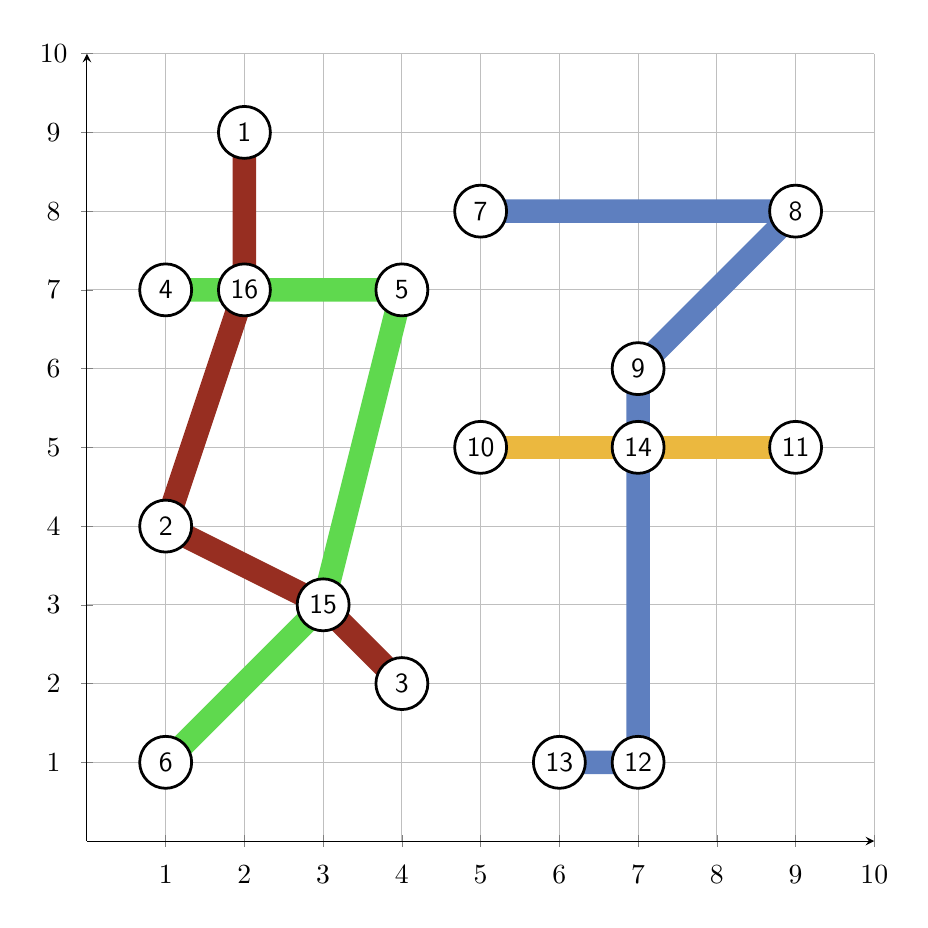
\begin{tikzpicture}[x=1cm,y=1cm,every node/.style={circle,inner sep=0pt,line width=1pt, minimum size = 0.66cm}]
		\begin{axis}[
			x=1.0cm,y=1.0cm,
			axis lines=middle,
			ymajorgrids=true,
			xmajorgrids=true,
			xmin=0,
			xmax=10,
			ymin=0,
			ymax=10,
			xtick={0.0,...,10.0},
			ytick={0.0,...,10.0},]	
			\begin{pgfonlayer}{foreground}
				\node[draw,fill=white] at (2cm,9cm) (v1) {1};
				\node[draw,fill=white] at (1cm,4cm) (v2) {2};
				\node[draw,fill=white] at (4cm,2cm) (v3) {3};
				\node[draw,fill=white] at (1cm,7cm) (v4) {4};
				\node[draw,fill=white] at (4cm,7cm) (v5) {5};
				\node[draw,fill=white] at (1cm,1cm) (v6) {6};
				\node[draw,fill=white] at (5cm,8cm) (v7) {7};
				\node[draw,fill=white] at (9cm,8cm) (v8) {8};
				\node[draw,fill=white] at (7cm,6cm) (v9) {9};
				\node[draw,fill=white] at (5cm,5cm) (v10) {10};
				\node[draw,fill=white] at (9cm,5cm) (v11) {11};
				\node[draw,fill=white] at (7cm,1cm) (v12) {12};
				\node[draw,fill=white] at (6cm,1cm) (v13) {13};
				\node[draw,fill=white] at (7cm,5cm) (v14) {14};
				\node[draw,fill=white] at (3cm,3cm) (v15) {15};
				\node[draw,fill=white] at (2cm,7cm) (v16) {16};
			\end{pgfonlayer}
			\draw[-,line width=0.3cm,line join=round,red] (v1.center) -- (v16.center) -- (v2.center) -- (v15.center) -- (v3.center);
			\draw[-,line width=0.3cm,line join=round,green] (v4.center) -- (v16.center) -- (v5.center) -- (v15.center) -- (v6.center);
			\draw[-,line width=0.3cm,line join=round,blue] (v7.center) -- (v8.center) -- (v9.center) -- (v14.center) -- (v12.center) -- (v13.center);
			\draw[-,line width=0.3cm,line join=round,yellow] (v10.center) -- (v14.center) -- (v11.center);
		\end{axis}
	\end{tikzpicture}
\end{document} 
